\chapter{Oprogramowanie}
W obecnych czasach praca w eksperymencie fizyki wysokich energii nieodzownie łączy się z programowaniem. Każdy element pracy zaczynając od zbierania danych poprzez selekcja przypadków po analizę wykonywany jest poprzez napisane przez członków kolaboracji oprogramowanie. Dlatego tak ważnym elementem w pracy są umiejętności programistyczne. Poniższy rozdział ma na celu przedstawienie narzędzi używanych podczas analizy, która to jest opisywana przez niniejszą pracę magisterską. Ponadto pokrótce przedstawione będą techniki tworzenia oprogramowania, na których autor starał się oprzeć swoje badania.

\section{Root}
Root \cite{ROOT} jest zorientowaną obiektową platformą programistyczną (ang. framework) napisaną w języku C++ na potrzeby Fizyki Wysokich Energii rozwijana przy ośrodku CERN, oraz rozpowszechniana na licencji LGPL. Głównymi zaletami środowiska są wysoce rozwinięte biblioteki ułatwiające statystyczną analizę danych. ROOT umożliwia między innymi:
\begin{itemize}
 \item tworzenie oraz analizę histogramów, zarówno jedno jak i wielowymiarowych,
 \item dopasowywania krzywych do danych przy użyciu różnych metod, między innymi metody największej wiarygodności, czy minimalizacji funkcji $\chi^2 $,
\item bardzo wydajne,pod względem ilości zajmowanego miejsca, przechowywanie danych, w tym celu utworzone i zoptymalizowane obiekty o nazwie Ntuple,
\item korzystanie z zaawansowanych operacji matematycznych np. rachunek na macierzach, czterowektorach,
\item równoległe przetwarzanie danych
\item prace z specjalnie stworzonym interpreterem 
\item wizualizację 3D
\item tworzenie plików w wielu najpopularniejszych formatach graficznych typu  PostScript, PNG, SVG, JPG czy GIF
 \end{itemize}
 \section{Gaudi}
 Eksperyment Fizyki Wysokich Energii produkuje rocznie peta bajty danych, które muszą zostać zebrane, a następnie przeanalizowane w celu produkcji końcowych fizycznych rezultatów. Czas życia takiego eksperymentu wynosi wiele lat w związku z tym oprogramowanie rozwijane przy nim musi mieć możliwość dopasowania do zmian technologii. Drugim ważnym wymaganiem dotyczącym oprogramowania jest elastyczność, możliwość wykorzystania w wielu dziedzinach, począwszy wydobycia interesujących przypadków z tła- algorytm HLT, poprzez rekonstrukcję po analizę fizyczną. Jednym z powodów owych wymagań jest ujednolicenia całego oprogramowania używanego przez ludzi pracujących przy eksperymencie, co ułatwia  zajmowanie się wieloma aspektami pracy, wystarczy jednorazowe nauczeniu się zasad tworzenia oprogramowania. 
 
Wychodząc na przeciw tym wymaganiom stworzono architekturę GAUDI\cite{GAUDI}. Podczas tworzenia architektury została podjęta decyzja o rozdzieleniu ``danych'' od ``algorytmów''. Poprzez dane rozumiano przykładowo składowe pędów oraz energie cząstek natomiast algorytmem może być funkcja wyliczająca masę inwariantną oraz dopasowująca odpowiednią krzywą. Algorytmy mogą tworzyć nowe typy danych. Natomiast dane dzielimy na trzy typy:
\begin{itemize}
 \item Event data - dane otrzymane z zderzenia protonów oraz ich pochodne,
 \item Detector - data opisujące aparaturę detekcyjną, używane do interpretowania danych pomiarowych ( struktura, geometria, parametry środowiskowe),
 \item Dane statystyczne - wynik przetwarzania ww danych (histogramy, Ntuple).
\end{itemize}
 \begin{figure}[h]
 \centering
 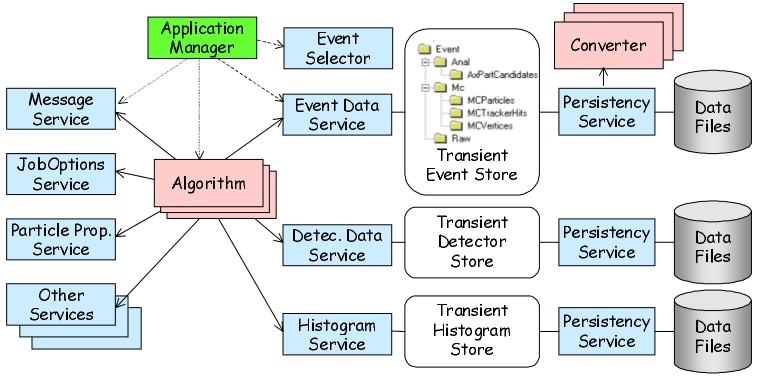
\includegraphics[scale=0.8]{rozdzial4/GAUDI.jpeg}
 % GAUDI.jpeg: 767x379 pixel, 96dpi, 20.29x10.03 cm, bb=0 0 575 284
 \caption{Schemat blokowy architektury GAUDI\cite{GAUDI}}
 \label{rys:GAUDI architektura}
\end{figure}

Rysunek \ref{rys:GAUDI architektura} przedstawia główne elementy architektury oraz ich interakcję, przy czym nie wchodzi w szczegóły dotyczące zastosowanych klas. \\
Dzięki swojej elastyczności GAUDI jest podstawą oprogramowania używanego w LHCb oraz ATLAS.
Kod źródłowy architektury GAUDI napisany jest w języku C++ to konfiguracja wykonywane jest przy użyciu skrpytów Python'owskich.

\subsection{Oprogramowanie LHCb}
Jak wcześniej wspomniano, większość oprogramowania używanego przez eksperyment LHCb bazuje na platformie programistycznej GAUDI. Oprogramowanie to składa się z wyspecjalizowanych aplikacji służących do symulacji, rekonstrukcji oraz analizy danych doświadczalnych. Poniżej znajduje się opis najważniejszych z nich, w szczególności z punktu widzenia niniejszej pracy magisterskiej.
\begin{itemize}
\item \textbf{Gauss} używany jest do symulacji Monte Carlo. Zawiera generator przypadków, jak również pozwala przeprowadzać symulacje oddziaływania z detektorem. Zderzenia proton-proton są symulowane przy wykorzystaniu programu PYTHIA\citep{PYTHIA}. Efekty detektorowe dodawane są dzięki użyciu pakietu GEANT4. 
\item \textbf{Boole} jego zadaniem jest symulacja odpowiedzi detektora oraz digitalizacje danych. Format danych generowanych przez ten program jest identyczny z tym, produkowanym przez elektronikę oraz system akwizycji danych. 
\item \textbf{Brunel} pozwala na rekonstrukcje przypadków na poziomie subdetektorów jak również na poziomie globalnym. Więcej o procesie rekonstrukcji można znaleźć w rozdziale poświęconym rekonstrukcji śladów. Ważną cechą jest możliwość przetwarzania danych wyprodukowanych przez Boole.
\item \textbf{DaVinci} jest to platforma programistyczna używana do fizycznej analizy pracująca w~ trybie offline. Pakiet ten jest bardzo istotny z punktu widzenia niniejszej pracy. Oprogramowanie odpowiedzialne za przetwarzanie danych, zarówno tych zebranych w trakcje pracy detektora jak i symulacji Monte Carlo, oraz tworzenie strumienia wyjściowego wykorzystywanego do dalszej analizy zostało stworzone jako część DaVinci'ego.
\item \textbf{Panoramix} jest zbiorem bibliotek umożliwiających wizualizacje przypadków.    
\end{itemize}
\section{Przetwarzanie sieciowe}
Ilość danych wytwarzanych przez detektory pracujące przy LHC jest tak wielka, że musiano stworzyć nową strategie przetwarzania ich. Strategia ta nazywana jest przetwarzaniem sieciowym lub GRID'owym. 

Grid dostarcza dwóch podstawowych funkcjonalności. Pierwszą z nich jest szybka dystrybucja danych pomiędzy centra przetwarzania danych umiejscowione na całym świecie. Druga natomiast związana jest z przydzielaniem zasobów systemowych w momencie uruchomienia przez użytkownika danego zadania. Dokładny opis realizacji tych zandań można znaleźć w \cite{Grid}.  W celu ułatwienia korzystania z rozproszonych zasobów stworzono interfejs Gaga\citep{Ganga}.

Przygotowanie danych oraz wstępna ich  analiza wykonana w ramach tej pracy magisterskiej została wykona przy użyciu przetwarzania GRID'owego. W celu uruchomienia zadania na sieci niezbędne było napisanie odpowiedniego skryptu python'owego tłumaczącego opcje DaVinci'ego, na zrozumiałe przez Gangę. Wykorzystanie rozproszonych zasobów pozwoliło to przeanalizować duże ilości danych. 

\section{System kontroli wersji}
W celu ułatwienia rozwoju oraz kontroli zmian w kodzie źródłowym podczas tworzenia oprogramowania do analizy posłużono się dwoma systemami kontroli wersji.
\begin{itemize}
\item \textbf{subversion} zwany również \textbf{svn} \cite{svn}.
\item \textbf{git} \cite{git}.
\end{itemize} 

